\documentclass{article}

\usepackage[T1]{fontenc}
\usepackage{amsmath}
\usepackage{amssymb}
\usepackage{mathtools}
\usepackage{algpseudocode}
\usepackage[inline]{enumitem}
\usepackage{listings}
\usepackage[framed]{matlab-prettifier}
\usepackage{pgfplots}
\usepackage[Polish]{babel}
\usepackage{float}

\DeclarePairedDelimiter{\norm}{\lVert}{\rVert}

\title{Sprawozdanie \\Metody numeryczne 2 \\\textbf{Temat 5, Zadanie nr 6}}
\date{28/12/2018}
\author{Mateusz Śliwakowski, F4}

\begin{document}
  \pagenumbering{gobble}
  \maketitle
 	  \newpage
  \pagenumbering{arabic}

\section{Treść zadania}
\paragraph{}
Odwrotna metoda potęgowa z normowaniem dla macierzy trójdiagonalnej. Poszukiwanie wartości własnej macierzy A leżącej najbliżej podanej wartości własnej $\lambda^*$. Układ równań z macierzą $A - \lambda^*I$ należy rozwiązać metodą dla macierzy trójdiagonalnych.
\section{Opis metody}
\subsection{Odwrotna metoda potęgowa}
\paragraph{}
Odwrotna metoda potęgowa korzysta z następującego twierdzenia:\\
\textit{Jeśli $\lambda$ jest wartością własną nieosobliwej macierzy $A$ to $\lambda^{-1}$ jest wartością własną macierzy $A^{-1}$.}
Polega ona na zastosowaniu metody potęgowej do macierzy $A^{-1}$.
\paragraph{}
Jeśli dobierzemy $\lambda^*$ takie, że $det(A-\lambda^{*}I)\neq0$ to $$\lambda \in \sigma(A) \Leftrightarrow \lambda \neq \lambda^{*} \wedge \frac{1}{\lambda-\lambda^{*}} \in \sigma(A-\lambda^* I)^{-1}$$ 
\paragraph{}
Zatem aby wyznaczyć wartość własną A, najbliższą danej $\lambda^*$, należy zastosować metodę potęgową do macierzy $(A-\lambda^*I)^{-1}$.\\
Ze względów wydajnościowych nie należy obliczać macierzy $(A-\lambda^*I)^{-1}$ (jest to kosztowna operacja). Pojedynczy krok metody potęgowej wykonujemy rozwiązując układ równań liniowych $(A - \lambda^*I)x^{(k)} = x^{(k-1)}$. Szczegółowy opis metody rozwiązywania tego układu zostanie opisany w następnej sekcji sprawozdania.
\subsection{Rozwiązywanie układu równań z macierzą trójdiagonalną}
\label{tridiagonal}
\paragraph{}
Mając macierz trójdiagonalną, nie jest optymalnym przechowywać ją całą w pamięci - lepszym rozwiązaniem jest zapisywanie trzech wektorów zawierających elementy kolejnych diagonali. Wygodnymi sposobami na rozwiązanie takich równań są m. in. metody iteracyjne, czy metoda Thomasa. Jednak na potrzeby zadania zdecydowałem się na zaimplementowanie metody GEPP dla tego szczególnego przypadku, ponieważ jest ona bardziej niezawodna niż wyżej podane.
\paragraph{}
Algorytm GEPP:\\
Załóżmy, że mamy daną macierz $A\in\mathbb{R}^{n\times n}$ - trójdiagonalna. Dla $k=1:n-1$:
\begin{enumerate}
\item Sprawdź czy $|A[k+1,k]| > |A[k,k]|$.
\item Jeśli tak to zamień wiersze $k+1$ i $k$-ty (w naszym przypadku zamieniamy elementy w wektorach).
\item Od wiersza $k+1$ odejmij $w_{k}*A[k+1,k]/A[k+1,k]$ (również posługujemy się operacjami na wektorach).
\end{enumerate}
Następnie obliczamy elementy wektora wynikowego korzystając z prostego algorytmu dla macierzy trójkątnej górnej.
\section{Warunki i założenia}
\begin{enumerate}
\item Wektory zawierające diagonalę mają poprawne rozmiary.
\item Macierz $A - \lambda^*I$ nie jest macierzą osobliwą.
\item $\lambda^*$ znajduje się wystarczająco blisko wartości własnej $A$. 
\end{enumerate}
\section{Implementacja}
Polecenie zadania realizuje funkcja \textit{pMethod}. Jej ciało nie jest obszerne, dlatego zamieszczam je poniżej:
\begin{lstlisting}[style=Matlab-editor]
function [lambda, iterations] = pMethod(v1, v2, v3, lambdaApproximation, precision, maxIterations)
n = size(v2,2);
v2 = v2 - lambdaApproximation*ones(1,n);

x_prev = rand(n,1);

lambdaPrev = lambdaApproximation;
lambda = lambdaApproximation + 2*precision; 
iterations = 0;

while(abs(lambda-lambdaPrev) >= precision)
    lambdaPrev = lambda;
    y_next = solveTridiagonal(v1,v2,v3,x_prev);
    s = dot(x_prev, y_next);
    lambda = 1/s + lambdaApproximation;
    x_prev = y_next/norm(y_next,2);
    
    iterations = iterations + 1;
    
    if(iterations > maxIterations)
        break;
    end
end
end
\end{lstlisting}
\vspace{4pt}
Parametry wejściowe:
\begin{itemize}
\item $v1, v2, v3$ - wektory zawierające diagonale, $v1$ zawiera diagonalę górną, $v2$ główną, a $v3$ dolną,
\item $lambdaApproximation$ - przybliżenie wartości własnej ($\lambda^*$),
\item $precision$ - zadana precyzja,
\item $maxIterations$ - maksymalna liczba iteracji, jaką może wykonać algorytm.
\end{itemize}
Parametry wyjściowe:
\begin{itemize}
\item $lambda$ - wyjściowa wartość własna - jeżeli algorytm zadziała poprawnie jest to wartość własna najbliższa $lambdaApproximation$,
\item $iterations$ - liczba iteracji, jaką wykonał algorytm.
\end{itemize}
\paragraph{}
Na początku odejmujemy od każdego elementu głównej diagonali wartość $lambdaApproximation$. Następnie losujemy przybliżenie początkowe i inicjalizujemy zmienne pomocnicze. Pętlę \textit{while} wykonujemy do uzyskania zadanej dokładności lub przekroczenia maksymalnej ilości iteracji. W jej wnętrzu wykonujemy algorytm zgodnie z opisem z sekcji \textit{Opis metody}.
\paragraph{}
Do rozwiązania układu równań $(A - \lambda^*I)x^{(k)} = x^{(k-1)}$ używamy funkcji \textit{solveTridiagonal}, która zaimplementowana jest zgodnie z opisem w punkcie \ref{tridiagonal}. Ponadto w celu ułatwienia przeprowadzania testów utworzyłem funkcje przydatne przy pracy z macierzami trójdiagonalnymi: \textit{createMatrixFromVectors} - tworzącą macierz kwadratową na podstawie danych wektorów oraz \textit{getThreeDiagonals} zwracającą 3 diagonale danej macierzy.
\section{Przykłady i wnioski}
\paragraph{}
Kod źródłowy przykładów opisanych poniżej znajduje się w plikach \textit{test.m} oraz \textit{iterationsTest.m}.
\subsection{Sprawdzenie poprawności działania funkcji}
Na początku sprawdzimy, czy nasza funkcja znajduje poprawną wartość własną dla danej macierzy. Aby uzyskać wszystkie wartości własne macierzy użyjemy wbudowanej funkcji \textit{eig}. Zacznijmy od prostej macierzy $4\times 4$, w postaci 
$$
\begin{bmatrix}
4 & 1 & 0 & 0\\
1 & 4 & 1 & 0\\
0 & 1 & 4 & 1\\
0 & 0 & 1 & 4
\end{bmatrix}
$$
Funkcja \textit{eig} zwróciła następujące wartości własne:\\
\begin{lstlisting}[style=Matlab-editor]
2.381966011250106
3.381966011250105
4.618033988749897
5.618033988749896
\end{lstlisting}
\vspace{4pt}
W celu wykonania testu weźmiemy przybliżenia początkowe będące zaokrągleniem podanych wartości własnych do liczby całkowitej. Ustalmy parametr \textit{precision} na $1e-6$. 
\begin{lstlisting}[style=Matlab-editor]
[lambdas(1), ~] = pMethod(v1,v2,v3, 2, 1e-6, 1e6);
[lambdas(2), ~] = pMethod(v1,v2,v3, 3, 1e-6, 1e6);
[lambdas(3), ~] = pMethod(v1,v2,v3, 5, 1e-6, 1e6);
[lambdas(4), ~] = pMethod(v1,v2,v3, 6, 1e-6, 1e6);
disp(eig(A) - lambdas)
\end{lstlisting}
\vspace{4pt}
Wynik:
\begin{lstlisting}[style=Matlab-editor]
   1.0e-06 *

  -0.013264893183873
  -0.394227355648979
   0.311422149401608
   0.030905391135150
\end{lstlisting}
\vspace{4pt}
Zarówno otrzymane wartości jak i dokładność są zgodne z oczekiwaniami.
\subsection{Sprawdzenie zbieżności dla macierzy o wartościach własnych bliskich sobie}
\paragraph{}
Aby w prosty sposób utworzyć macierz trójdiagonalną o wartościach własnych bliskich sobie, skorzystamy z faktu, że macierze podobne mają te same wartości własne oraz ograniczymy się do macierzy $2\times 2$. Ponadto, warto przypomnieć fakt, że wartości własne macierzy diagonalnej to wartości leżące na diagonali tej macierzy. Weźmy zatem macierz: 
$$T = \begin{bmatrix}
1.0001 & 0\\
0 & 1.0002
\end{bmatrix}$$
Wygenerujmy losowo macierz B. Macierz do naszych testów to $A = BTB^{-1}$. Dla porównania sprawdzimy jak zachowa się funkcja dla macierzy $A' = BT'B^{-1}$, gdzie:
$$T' = \begin{bmatrix}
1.0001 & 0\\
0 & 2
\end{bmatrix}$$
Pozostałe parametry pozostawimy bez zmian. Dla przybliżenia początkowego równego 1:\\
\vspace{4pt}
\begin{tabular}{ | l | l | l |}
    \hline
    dokładność & iteracje dla $T$ & iteracje dla $T'$\\ \hline
    $1e-6$ & 23 & 7 \\ \hline
    $1e-8$ & 34 & 13\\ \hline
    $1e-10$ & 35 & 16\\ \hline
    $1e-12$ & 39 & 26\\ 
    \hline
\end{tabular}\\
Dla przybliżenia początkowego równego 0.5:\\\\
\begin{tabular}{ | l | l | l |}
    \hline
    dokładność & iteracje dla $T$ & iteracje dla $T'$\\ \hline
    $1e-6$ & 3 & 13 \\ \hline
    $1e-8$ & 3991 & 19\\ \hline
    $1e-10$ & 23962 & 20\\ \hline
    $1e-12$ & 52052 & 26\\ 
    \hline
\end{tabular}\\\\
Faktycznie, ilość iteracji jest dużo wyższa dla macierzy o wartościach własnych bliskich sobie. Fakt ten widoczny jest zwłaszcza, gdy weźmiemy przybliżenie początkowe, nie znajdujące się blisko wartości własnej.
\subsection{Zależność ilości wykonanych iteracji od zadanej dokładności}
\paragraph{}
W ostatnim kroku przetestujemy, jak zwiększa się ilość iteracji w zależności od zadanej dokładności, dla macierzy o współczynnikach wybranych losowo.
\begin{figure}[H]
  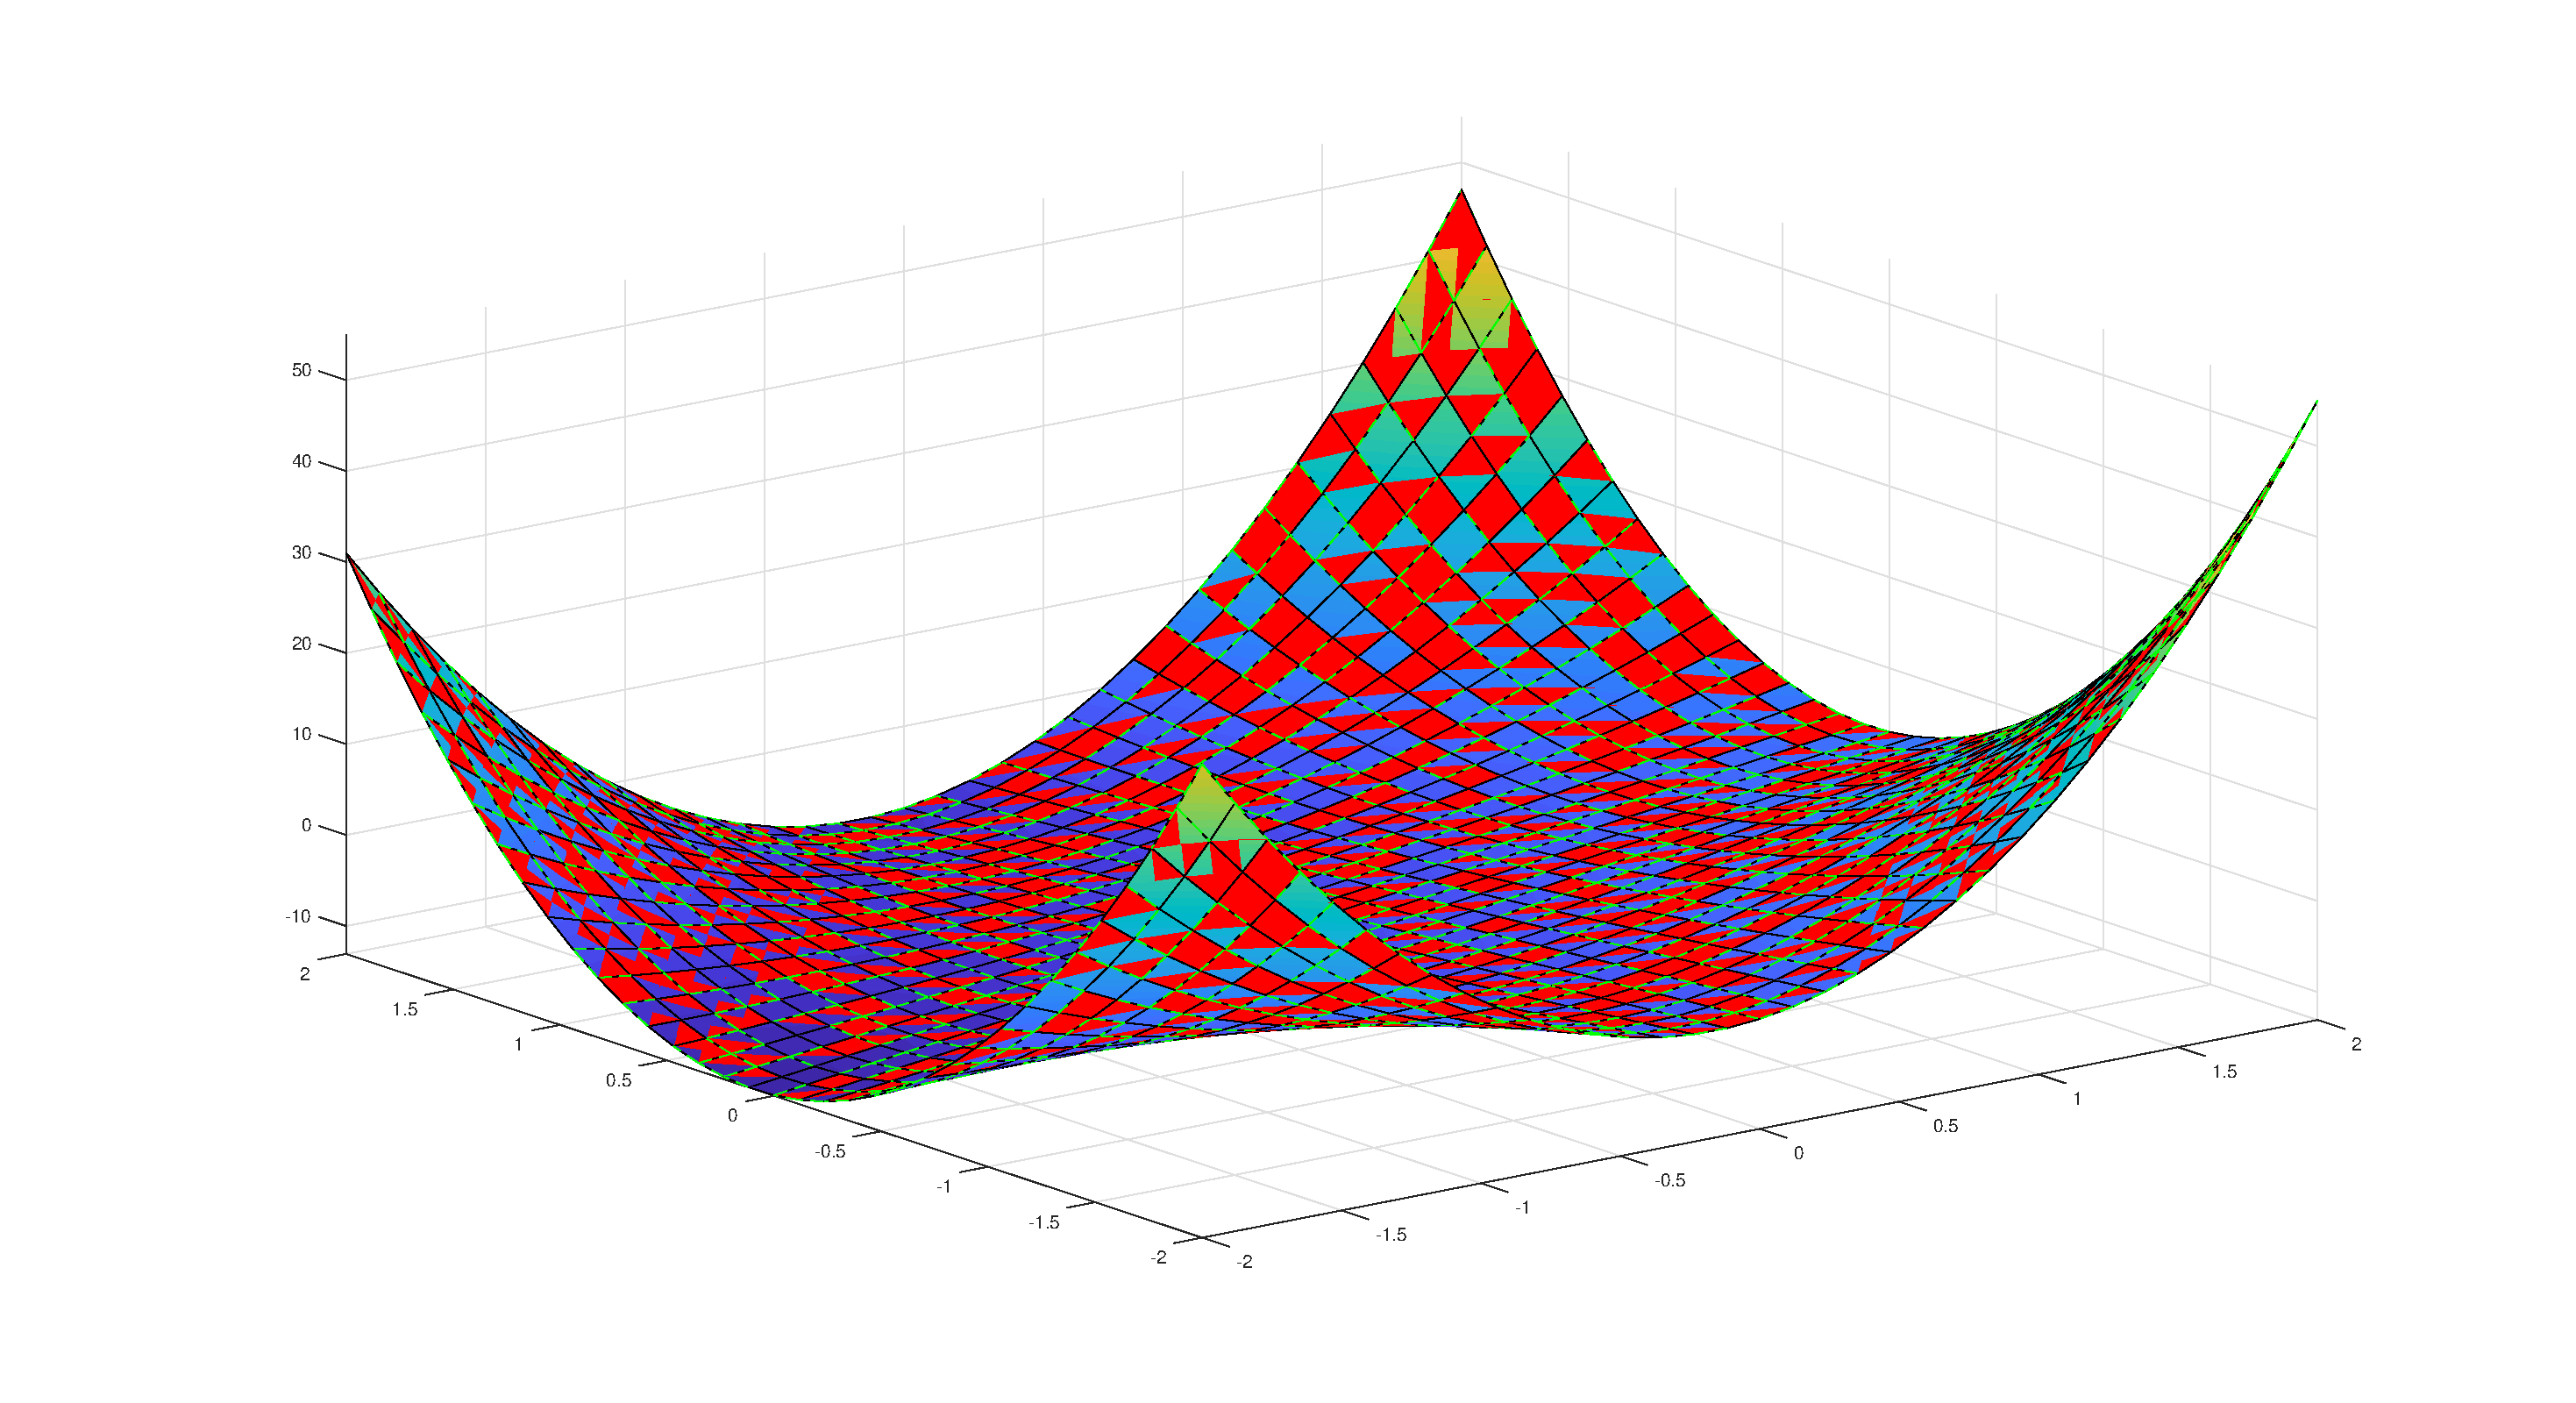
\includegraphics[width=\linewidth]{fig1.eps}
\end{figure}
\paragraph{}
Można zauważyć, że zwiększanie dokładności o rząd wielkości powoduje wzrost liczby iteracji o stałą wartość (w tym przypadku pomiędzy 4, a 5).
\subsection{Wnioski}
\begin{itemize}
\item Algorytm działa poprawnie - jeśli podamy przybliżenie różne od wartości własnej i znajdujące się dostatecznie blisko niej, to otrzymamy poprawny wynik.
\item Metoda jest wolno zbieżna, jeżeli wartości własne macierzy znajdują się blisko siebie. Efekt ten jest spotęgowany, kiedy wybierzemy przybliżenie początkowe dalekie dokładnej wartości własnej.
\item Liczba iteracji rośnie o stałą wartość wraz ze wzrostem dokładności o rząd wielkości - możemy zatem zwiększać dokładność niewielkim kosztem.
\end{itemize}
\end{document}